\section{Evaluation-Driven Development: Formative Prototype Evaluation during Development}

% ---------------------------------------------------------------------------------------------------------------------
\subsection{Implementation Procedure}
\label{sec:evaluation-driven-development}

Die Entwicklung des Prototyps folgte dem Evaluation-Driven Development (EDD) Ansatz (vgl.
\autoref{sec:evaluation-driven-development}). Dabei kamen bereits während der Implementierung automatisierte
Prüfverfahren zum Einsatz, um das System kontinuierlich zu evaluieren.

Nutzerstudien, Human-in-the-Loop-Evaluierungen oder Expertenbewertungen waren in dieser frühen Prototyping-
und Entwicklungsphase nicht praktikabel, da solche Verfahren ohne erheblichen Aufwand nicht skalierbar sind.
Stattdessen erfolgte die Weiterentwicklung des Systems in kurzen Zyklen aus Implementierung, Prüfung und
Anpassung. Dieses iterative Vorgehen ist in der Softwareentwicklung etabliert (vgl.
\cite[p.~8]{ottAppsEffektivManagen2019}) und besonders bei EDD von KI-basierter Systeme relevant, da aufgrund
der vielfältigen Nutzungsmöglichkeiten hier kein vollständiges Testorakel vorausgesetzt werden kann
\cite[p.~39]{istqbrISTQBCertifiedTester}.

Für Komponenten, die nicht auf probabilistische KI-Modellausgaben angewiesen waren, sowie Unit- und
Integrationstests, kamen klassische Softwaretests zum Einsatz, da sich für diese ein eindeutiges und
deterministisch prüfbares Testorakel definieren ließ. Da der überwiegende Teil des zu testenden Systems
jedoch auf LLM-basierte Komponenten angewiesen und somit probabilistisch ist, war dies in den meisten Fällen
nicht möglich.

Deshalb wurde ein von der Methode „LLM-as-a-Judge“ inspirierter Ansatz gewählt (vgl.
\autoref{sec:llm-as-a-judge}). In der hier verwendeten Version bewertete das LLM den Output nicht in
Echtzeit, sondern wurde genutzt um im Voraus Szenarien (meist mögliche Konversationen) für spezifische
Situationen zu generieren, um ein lexikalisches Testorakel zu erstellen. Dieses wurde im Rahmen
codebasierter (vgl. \autoref{sec:code-based-testing}) automatiserierter Test, in Kombination mit regulären
Ausdrücke verwendet.
Das vom LLM-Judge genereierte Orakel operationalisierte, welche Formulierungen eine fachlich angemessene
Facilitator-Äußerung in dem jeweiligen Szenario aufweisen muss und welche sie nicht aufweisen darf. Der Output
der einzelnen Komponenten wurde überwacht und analysiert, um das Verhalten der Komponenten in den
verschiedenen Szenarien besser verstehen und bewerten zu können.

Während der Entwicklung wurde das System kontinuierlich in unstrukturierten, explorativen Tests,
sowohl einzeln als auch unregelmäßig mit mehreren Personen in verschiedenen, nicht weiter spezifizierten
Szenarien überprüft. Ziel war es, bereits vor den eigentlichen Nutzerstudien (vgl.
\autoref{ch:empirical-prototype-validation}) ein Gefühl für das Systemverhalten zu entwickeln. Dadurch
sollten offensichtliche Fehler sowie kritische Schwachstellen, an denen das System vom intendierten
Verhalten abweicht, frühzeitig erkannt werden, um das System anzupassen.

Dieses Vorgehen kann in einem Loop wie folgt dargestellt werden:

\begin{figure}[H]
  \centering
  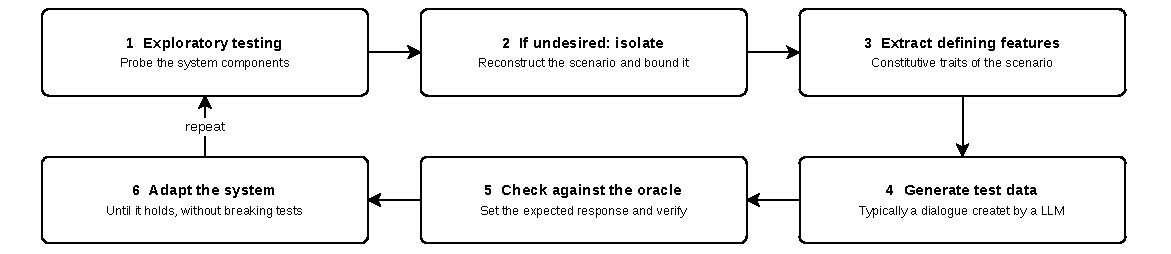
\includegraphics[width=\textwidth]{assets/figures/04/evaluation-driven-development-loop.pdf}
  \caption{Evaluation-driven development loop: From exploratory testing to system adaptation
  \figsource{Own illustration, created with draw.io.}}
  \label{fig:evaluation-driven-development-loop}
\end{figure}

Das sukzessive erweiterte Testorakel diente zugleich als Regressionstest, um zu erkennen ob eine Systemänderung
zuvor gesichertes Verhalten nicht beeinträchtigt.

\label{sec:langfuse}
Zum genaueren monitoren des Systems wurde zusätzlich zu den automatisierten Tests Langfuse genutzt.
Langfuse ist eine Open-Source-Plattform zur Observability und Evaluation von LLM-Anwendungen, die
Trace-Level-Daten zu Modellaufrufen, Prompts und Nutzerinteraktionen erfasst und deren Analyse, Bewertung
sowie kontinuierliche Optimierung ermöglicht. \cite{LangfuseOpenSource}

\begin{figure}[H]
  \centering
  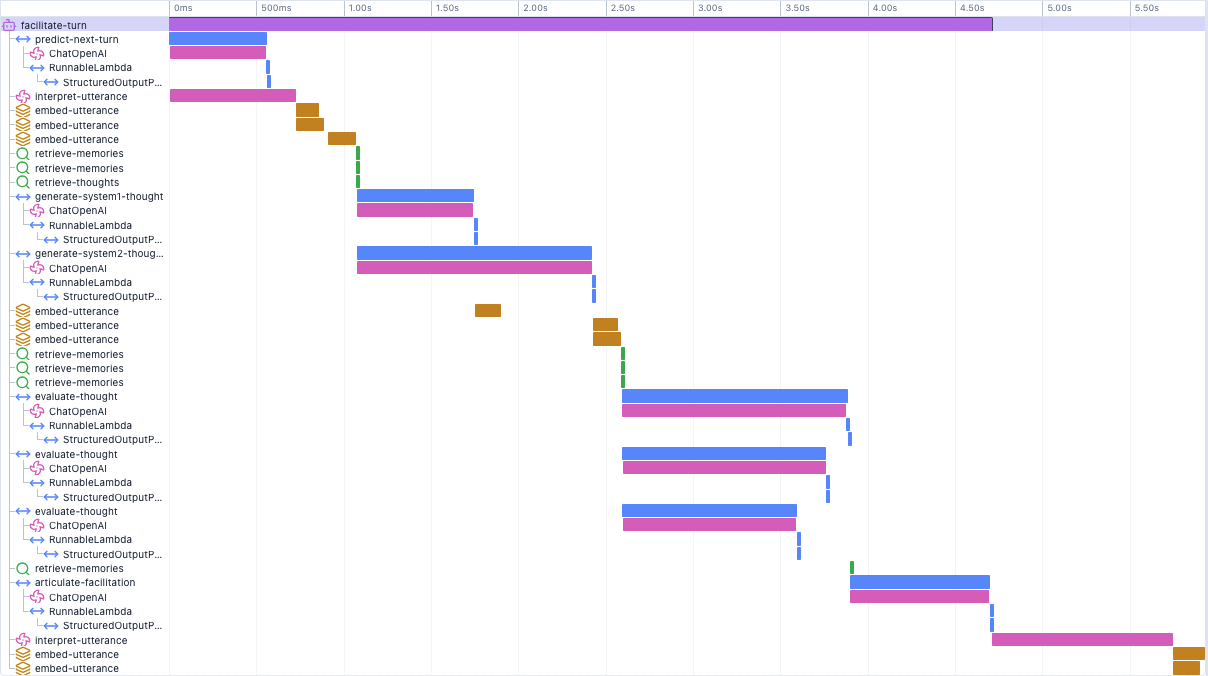
\includegraphics[width=0.99\textwidth]{assets/figures/04/langfuse-traceview-screenshot.png}
  \caption{Langfuse: Screenshot of the Traceviewer in Langfuse that shows the trace of the AI-Facilitator
    processing a new conversation event.
  \figsource{Own screenshot, created with Langfuse.}}
  \label{fig:langfuse}
\end{figure}

\subsection{Limitierungen des Vorgehens}
\label{sec:edd-limitations}

Ein lexikalisches Orakel ist unvollständig und die qualität hängt in diesem Fall von dem LLM-Judge ab.
Eine gültige Facilitator-Äußerung kann das intendierte Verhalten zeigen, ohne die vorgesehenen
Wortgruppen zu enthalten; umgekehrt kann ein Treffer formal korrekt und situativ unpassend sein.
Isolierte Dialoge blenden zudem die Dynamik eines echten Meetings aus: Turn-Taking, Timing und die
Reaktion der Gruppe auf eine Intervention bleiben unberücksichtigt.
Welche Szenarien überhaupt als Testdaten aufgenommen wurden, hängt außerdem von den explorativ
beobachteten Fehlern ab und ist damit autorenseitig selektiert.

Dennoch entspricht diese Kombination, von kontinuierliche, orakelgestützte Prüfung während der Implementierung und
unabhängige Human-in-the-Loop-Evaluation danach (druch die User Studien), einem valider Ansatz zum prüfen von
llm basierten agentischen Systemen.
\cite[pp.~6--7]{mohammadiEvaluationBenchmarkingLLM2025}.

% Während der Entwicklungsphase ist es unpraktisch, für jede Code-Änderung oder Anpassung von Parametern
% Nutzerstudien durchzuführen. Die Autoren von Inner Thoughts schlagen dafür eine Multi-Agenten-Simulation vor.
% \cite["6 Simulative Evaluation"]{liuProactiveConversationalAgents2025}
% Dabei wurden in diesem verschiedene Thoughtful Agents mit den unterschiedklciehn Infromationen und Profilen
% aus dem hidden-Profiles experiment ausgestattet, sodass der Gesprächsverlauf zwischen den KI-Agenten
% simuliert werden kann. Während der Entwicklung wird dabei
% ausschließlich die Moderationsstrategie des AI-Facilitators variiert bzw. optimiert.

% Es wirde die Einschätzung von Liu et al. geteilt, dass eine solche Simulation skalierbar ist und sich
% Fehler im Moderationsverhalten (z.B. unpassendes Timing oder Unterbrechungen) über längere Interaktionen
% hinweg akkumulieren und verstärken \cite["6 Simulative Evaluation"]{liuProactiveConversationalAgents2025}.
% Ein schlechtes Systemdesign, ungeeignete Prompts oder Parameter sollten demnach zu einer erkennbar
% schlechteren Gesprächsqualität führen.

% Für die Evaluierung der Gesprächs- bzw. Moderationsqualität käme ein menschlicher Bewerter in Form von
% Facilitating-Experten infrage.
% Da das ausgewählte Hidden-Profile-Verfahren jedoch etwa 30 Minuten dauert, ist dies während der
% Entwicklungsphase kaum praktikabel, weil die Aussagekraft der Evaluierung mit jeder weiteren Anpassung des
% Systems abnimmt und die Systemausgaben nach jeder Modifikation erneut aufwändig bewertet werden müssten.

% Aus diesem Grund wurde ein LLM-as-a-Judge-Ansatz mit einer G-Eval-Replikation gewählt, der die allgemeine
% Meetingqualität basierend auf dem Fragebogen von XY abgeleitetn Kriteren bewerten sollte.

% Zusätzlich evaluierte ein weiteres LLM, ob die Teilnehmer alle relevanten Informationen von den Steckbriefen
% genannt hatten. Diese Klassifizierung wurde anschließend statistisch ausgewertet.

% Darüber hinaus wurden mithilfe von LLMs Gesprächsszenarien systematisch generiert, in denen ein Facilitator
% eingreifen würde. Ziel war es, das "External Stimulus Injection Layer" zu überprüfen. Dabei wurde analysiert,
% wie häufig der AI-Facilitator an den erwarteten Stellen aufgrund des gesetzten External Stimulus eingriff.
% Diese automatisierten Tests wurden während des Systemdesigns und der Entwicklung regelmäßig durchgeführt,
% sobald der Autor eine Änderung vorgenommen hatte, von der er sich eine Verbesserung erhoffte.

% Somit wurde versucht sich bassierend auf diesen Tests zu qualifizieren ob die Entwicklung eines Moderation
% System in eine Richtung geht, die die Qualität des Meetings in einer hiddenprofile konstelation verbessert.

% Um die aussagekraft in realen Bedinung mit Menschen zu evaluieren wurden nach der Entiwkclungsphase
% Usability-Studien durchgeführt.
% (vgl. Section XYZ TODO)
